\documentclass{article}
\usepackage{graphicx}
\usepackage{xcolor}
	\pagecolor{black}%
\color{white}%
\title{5 PROGRAMMING LANGUAGES AND THEIR HISTORICAL PERSPECTIVES BY NNADIUKWU MIRACLE}
\begin{document}
	\pagenumbering{gobble}
	\maketitle
	\newpage
	\pagecolor{black!2}
		\color{black}
	\pagenumbering{arabic}
	\centering
	
	\section*{JAVASCRIPT}
	
	\begin{figure}
		\begin{center}
			\pagecolor{black!3}
			\color{black}
			
\includegraphics[width=0.3\linewidth]{js.png}
			\end{center}
	\end{figure}
	\begin{itemize}
		\item JavaScript often abbreviated as JS, is a programming language that conforms to the ECMAScript specification.
		\item JavaScript is high-level, often just-in-time compiled, and multi-paradigm. 
		\item Alongside HTML and CSS, JavaScript is one of the core technologies of the World Wide Web. 
		\item Over 97 per cent of websites use it client-side for web page behavior, often incorporating third-party libraries. 
		\item Most web browsers have a dedicated JavaScript engine to execute the code on the user's device.
			\end{itemize}
			\newpage
				\pagecolor{black}
			\color{white}
		\section*{BRIEF HISTORY OF JAVASCRIPT}
		\begin{itemize}
			\item JavaScript was created at Netscape Communications by Brendan Eich in 1995. 
			\item Netscape and Eich designed JavaScript as a scripting language for use with the company's flagship web browser, Netscape Navigator. 
			\item Initially known as Live Script, Netscape changed the name to JavaScript so they could position it as a companion for the Java language, a product of their partner, Sun Microsystems.
			\item After its release, more and more browsers started adding JavaScript support. 
			\item In 2008, the creation of Google's open-source Chrome V8, a high-performance JavaScript engine, provided a crucial turning point for JavaScript. 
			\item The subsequent proliferation of fast JavaScript engines made it possible for developers to build sophisticated browser-based applications with performance that competed with desktop and mobile applications.
			\item Soon after, Ryan Dahl released an open-source, cross-platform environment called Node.js. It provided a way to run JavaScript code from outside a browser. It freed JavaScript from the browser's confines and led directly to JavaScript's current popularity. Today, you can use JavaScript to write all kinds of applications, including browser, server, mobile, and desktop applications. 
	\end{itemize}
	\newpage
	\section*{FOUNDER OF JAVASCRIPT}
		\begin{itemize}
		\item Brendan Eich grew up in Pittsburgh; Gaithersburg, Maryland; and Palo Alto
		\item Attended Ellwood P. Cubberley High School, graduating in the class of 1979.
		\item He received his bachelor's degree in mathematics and computer science at Santa Clara University
		\item Received his master's degree in 1985 from the University of Illinois at Urbana–Champaign.
		\item He began his career at Silicon Graphics, working for seven years on operating system and network code.
		\item He then worked for three years at Micro Unity Systems Engineering writing microkernel and DSP code.
	\end{itemize}
\begin{figure}
		\begin{center}
	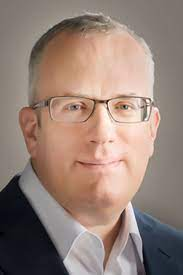
\includegraphics[width=0.4\linewidth]{brendan.jpg}
\end{center}
\end{figure}
		\newpage
	\section*{APPLICATIONS THAT CAN BE DEVELOPED FROM JAVASCRIPT}
	\paragraph{Applications that can be developed with JavaScript includes the following:
	}
\begin{itemize}
	\item Netflix
	\item Candy crush
	\item Uber
	\item LinkedIn
	\item Facebook etc.
\end{itemize}
\newpage
	\section*{IDE’s FOR JAVASCRIPT}
	\paragraph{The Integrated Development Environments for JavaScript includes the following:}
	\begin{itemize}
		\item Web storm
		\item Visual Studio Code
		\item Atom
		\item Sublime text
		\item NetBeans etc.
\end{itemize}
\newpage
\section*{PROGRAMMING LANGUAGES RELATED TO JAVASCRIPT}
\paragraph{These include:
}
\begin{itemize}
	\item Dart
	\item Typescript
	\item Elm
	\item Prescript
	\item Coffee script etc.
\end{itemize}

	\newpage
	\pagecolor{white}
	\color{black}
		\section*{HTML}
	\begin{itemize}
		\item The Hyper Text Markup Language, or HTML is the standard markup language for documents designed to be displayed in a web browser.
		\item It can be assisted by technologies such as Cascading Style Sheets (CSS) and scripting languages such as JavaScript.
		\item Web browsers receive HTML documents from a web server or from local storage and render the documents into multimedia web pages.
		\item HTML describes the structure of a web page semantically and originally included cues for the appearance of the document.
	\end{itemize}
\begin{figure}
		\begin{center}
	
\includegraphics[width=0.3\linewidth]{html.png}
\end{center}
\end{figure}
	\newpage
	\pagecolor{black}
	\color{white}
	\section*{BRIEF HISTORY OF HTML}
	\begin{itemize}
		\item HTML was created by Sir Tim Berners-Lee in late 1991 but was not released officially, published in 1995 as HTML 2.0. HTML 4.01 was published.
		\item HTML 1.0 was released in 1993 with the intention of sharing information that can be readable and accessible via web browsers. But not many of the developers were involved in creating websites. So the language was also not growing.
		\item HTML 2.0, published in 1995, which contains all the features of HTML 1.0 along with that few additional features, which remained as the standard markup language for designing and creating websites until January 1997 and refined various core features of HTML.
		\item HTML 3.0, where Dave Raggett who introduced a fresh paper or draft on HTML. It included improved new features of HTML, giving more powerful characteristics for webmasters in designing web pages. But these powerful features of new HTML slowed down the browser in applying further improvements.
		\item Then comes HTML 4.01, which is widely used and was a successful version of HTML before HTML 5.0, which is currently released and used worldwide. HTML 5 can be said for an extended version of HTML 4.01, which was published in the year 2012.
		in late 1999 and was a major version of HTML.
	\end{itemize}
	\newpage
	\section*{FOUNDER OF HTML}
	\begin{itemize}
		\item Berners-Lee was born on 8 June 1955 in London, England.
		\item The eldest of the four. His parents were computer scientists who worked on the first commercially built computer, the Ferranti Mark 1.
		\item He attended Sheen Mount Primary School, and then went on to attend south-west London's Emanuel School from 1969 to 1973, at the time a direct grant grammar school, which became an independent school in 1975.
		\item A keen trains potter as a child, he learnt about electronics from tinkering with a model railway.
		\item He studied at The Queen's College, Oxford, from 1973 to 1976, where he received a first-class Bachelor of Arts degree in physics.
		While at university, Berners-Lee made a computer out of an old television set, which he bought from a repair shop.
	\end{itemize}
	\begin{figure}
			\begin{center}
		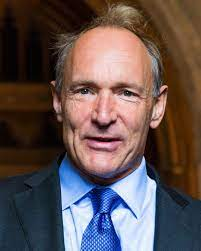
\includegraphics[width=0.3\linewidth]{tim.jpg}
	\end{center}
	\end{figure}
	\newpage
	\section*{APPLICATIONS THAT CAN BE DEVELOPED FROM HTML}
	\paragraph{Applications that can be developed with HTML includes the following:
	}
	\begin{itemize}
		\item Zoho
		\item Google docs
		\item Scribd
		\item Hoot suite
		\item Angry birds
		
	\end{itemize}
	\newpage
	\section*{IDE’s FOR HTML}
	\paragraph{The Integrated Development Environments for HTML includes the following:}
	\begin{itemize}
		\item Atom
		\item Komodo edit
		\item PHP storm
		\item Adobe Dreamweaver etc.
		
	\end{itemize}
	\newpage
	\section*{PROGRAMMING LANGUAGES RELATED TO HTML}
	\paragraph{These include:
	}
	\begin{itemize}
		\item Cascading Sheet Style
		\item JavaScript
		\item Hyper Text Processor etc.
	\end{itemize}

\newpage
\pagecolor{black!98}
\color{white}
\section*{PYTHON}
\begin{itemize}
	\item Python is an interpreted high-level general-purpose programming language. 
	\item Its design philosophy emphasizes code readability with its use of significant indentation. 
	\item Its language constructs as well as its object-oriented approach aim to help programmers write clear, logical code for small and large-scale projects.
	\item Python is dynamically-typed and garbage-collected.
	\item It supports multiple programming paradigms, including structured (particularly, procedural), object-oriented and functional programming.
\end{itemize}
\begin{figure}
		\begin{center}
	
\includegraphics[width=0.8\linewidth]{python.jpg}
\end{center}
\end{figure}
\newpage
\section*{BRIEF HISTORY OF PYTHON}
\begin{itemize}
	\item Python was conceived in the late 1980s by Guido van Rossum at Centrum Wiskunde and Informatica (CWI) in the Netherlands as a successor to ABC programming language, which was inspired by SETL, capable of exception handling and interfacing with the Amoeba operating system. 
	Its implementation began in December 1989.
	\item Van Rossum shouldered sole responsibility for the project, as the lead developer, until 12 July 2018.
	In January 2019, active Python core developers elected a five-member "Steering Council" to lead the project.
	\item Python 2.0 was released on 16 October 2000, with many major new features, including a cycle-detecting garbage collector and support for Unicode.
	\item Python 3.0 was released on 3 December 2008. It was a major revision of the language that is not completely backward-compatible.
	\item Many of its major features were backported to Python 2.6.x and 2.7.x version series. Releases of Python 3 include the 2to3 utility, which automates the translation of Python 2 code to Python 3.
	\item Python 2.7's end-of-life date was initially set at 2015 then postponed to 2020 out of concern that a large body of existing code could not easily be forward-ported to Python 3. No more security patches or other improvements will be released for it.
	\item Python 3.9.2 and 3.8.8 were expedited as all versions of Python (including 2.7) had security issues, leading to possible remote code execution and web cache poisoning.
\end{itemize}
\newpage
\section*{FOUNDER OF PYTHON}
\begin{itemize}
	\item Guido van Rossum; born 31 January 1956) is a Dutch programmer best known as the creator of the Python programming language, for which he was the "benevolent dictator for life" (BDFL) until he stepped down from the position in July.
	\item Van Rossum was born and raised in the Netherlands.
	received a master's degree in mathematics . 
	\item Also received a master’s degree in computer science from the University of Amsterdam in 1982.
	\item He has a brother, Just van Rossum, who is a type designer and programmer who designed the typeface used in the "Python Powered" logo.
	\item Van Rossum lives in Belmont, California, with his wife, Kim Knapp, and their son
	
\end{itemize}
\begin{figure}
		\begin{center}
	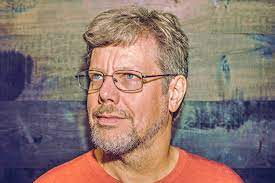
\includegraphics[width=0.4\linewidth]{guido.jpg}
\end{center}
\end{figure}
\newpage
\section*{APPLICATIONS THAT CAN BE DEVELOPED FROM PYTHON}
\paragraph{Applications that can be developed with PYTHON includes the following:
}
\begin{itemize}
	\item Pinterest
	\item Disqus
	\item Spotify
	\item Dropbox
	\item Uber
	\item Reddit etc.
\end{itemize}
\newpage
\section*{IDE’s FOR PYTHON}
\paragraph{The Integrated Development Environments for PYTHON includes the following:}
\begin{itemize}
	\item PY Charm
	\item Spyder
	\item IDLE
	\item Microsoft Visual Code etc.
	
	
\end{itemize}
\newpage
\section*{PROGRAMMING LANGUAGES RELATED TO PYTHON}
\paragraph{These include:
}
\begin{itemize}
	\item Java
	\item JavaScript
	\item Perl
	\item Tcl
	\item Smalltalk
	\item C++ etc.
\end{itemize}
\newpage
\pagecolor{white}
\color{black}
\section*{PHP}
\begin{itemize}
	\item PHP is a general-purpose scripting language geared towards web development.
	\item PHP originally stood for Personal Home Page, but it now stands for the recursive initialism PHP: Hypertext Preprocessor.
	\item PHP code is usually processed on a web server by a PHP interpreter implemented as a module, a daemon or as a Common Gateway Interface (CGI) executable. 
	\item On a web server, the result of the interpreted and executed PHP code – which may be any type of data, such as generated HTML or binary image data – would form the whole or part of an HTTP response.
	\item Additionally, PHP can be used for many programming tasks outside the web context, such as standalone graphical applications and robotic drone control. 
	\item PHP code can also be directly executed from the command line.	
\end{itemize}
\begin{figure}
		\begin{center}
	
\includegraphics[width=0.3\linewidth]{php.png}
\end{center}
\end{figure}
\newpage
\pagecolor{black}
\color{white}
\section*{BRIEF HISTORY OF PHP}
\begin{itemize}
	\item PHP was conceived sometime in the fall of 1994 by Rasmus Lerdorf.
	\item Early non-released versions were used on his home page to keep track of who was looking at his online resume. The first version used by others was available sometime in early 1995 and was known as the Personal Home Page Tools.  
	\item The parser was rewritten in mid-1995 and named PHP/FI Version 2. The FI came from another package Rasmus had written which interpreted html form data. He combined the Personal Home Page tools scripts with the Form Interpreter and added mSQL support and PHP/FI was born. PHP/FI grew at an amazing pace and people started contributing code to it.
	\item By late 1996 PHP/FI was in use on at least 15,000 web sites around the world.
	\item By mid-1997 this number had grown to over 50,000. 
	\item Mid-1997 also saw a change in the development of PHP. It changed from being Rasmus' own pet project that a handful of people had contributed to, to being a much more organized team effort. The parser was rewritten from scratch by Zeev Suraski and Andi Gutmans and this new parser formed the basis for PHP Version 3.
	\item Today, either PHP/FI or PHP3 ships with a number of commercial products such as C2's StrongHold web server and Red Hat Linux. A conservative estimate based on an extrapolation from numbers provided by \item Net Craft would be that PHP is in use on over 1,000,000 sites around the world.
	
\end{itemize}
\newpage
\pagecolor{black}
\color{white}
\section*{FOUNDER OF PHP}
\begin{itemize}
	\item Rasmus Lerdorf (born 22 November 1968) is a Danish-Canadian programmer. 
	\item He co-authored and inspired the PHP scripting language, authoring the first two versions of the language and participating in the development of later versions led by a group of developers.
	\item Lerdorf was born on Disko Island in Greenland and moved to Denmark in his early years. 
	\item He graduated from King City Secondary School in 1988 
	\item In 1993, he graduated from the University of Waterloo with a Bachelor of Applied Science in Systems Design Engineering. 
	\item He contributed to the Apache HTTP Server and he added the LIMIT clause to the mSQL DBMS. A variant of this LIMIT clause had already been around for a decade in mainframe relational database management systems (like Oracle Rdb running on VAX/VMS, formerly from Digital Equipment Corporation), but apparently it had not yet been picked up by the emerging PC-based databases. It was later adapted by several other SQL-compatible DBMS. 
	\item  released the first version of PHP in 1995.
\end{itemize}
\begin{figure}
		\begin{center}
	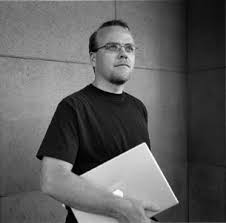
\includegraphics[width=0.4\linewidth]{rasmus.jpg}
\end{center}
\end{figure}
\newpage
\section*{APPLICATIONS THAT CAN BE DEVELOPED FROM PHP}
\paragraph{Applications that can be developed with PHP includes the following:
}
\begin{itemize}
	\item Facebook
	\item Yahoo
	\item Wikipedia
	\item WordPress
	\item Mail Chimp
	\item Digg etc.
\end{itemize}
\newpage
\section*{IDE’s FOR PHP}
\paragraph{The Integrated Development Environments for PHP includes the following:}
\begin{itemize}
	\item PHP Storm
	\item Code Lobster
	\item NetBeans
	\item Komodo IDE etc.
\end{itemize}
\newpage
\section*{PROGRAMMING LANGUAGES RELATED TO PHP}
\paragraph{These include:
}
\begin{itemize}
	\item JS. Node
	\item Python
	\item Ruby
	\item Golang
	\item Java
	\item C sharp etc.
\end{itemize}
\newpage
\pagecolor{white}
\color{black}
\section*{SWIFT}
\begin{itemize}
		\item Swift is a general-purpose, multi-paradigm, compiled programming language developed by Apple Inc. and the open-source community. 
	\item First released in 2014, Swift was developed as a replacement for Apple's earlier programming language Objective-C, as Objective-C had been largely unchanged since the early 1980s and lacked modern language features. 
	\item Swift works with Apple's Cocoa and Cocoa Touch frameworks, and a key aspect of Swift's design was the ability to interoperate with the huge body of existing Objective-C code developed for Apple products over the previous decades. 
	\item It is built with the open source LLVM compiler framework and has been included in Xcode since version 6, released in 2014. On Apple platforms, it uses the Objective-C runtime library, which allows C, Objective-C, C++ and Swift code to run within one program.
\end{itemize}
\begin{figure}
		\begin{center}
	
\includegraphics[width=0.3\linewidth]{swift.jpg}
\end{center}
\end{figure}
\newpage
\pagecolor{black}
\color{white}
\section*{BRIEF HISTORY OF SWIFT}
\begin{itemize}
	\item Development of Swift started in July 2010 by Chris Lattner, with the eventual collaboration of many other programmers at Apple.
	\item On June 2, 2014, the Apple Worldwide Developers Conference (WWDC) application became the first publicly released app written with Swift.
	\item A beta version of the programming language was released to registered Apple developers at the conference, but the company did not promise that the final version of Swift would be source code compatible with the test version.
	\item Swift reached the 1.0 milestone on September 9, 2014, with the Gold Master of Xcode 6.0 for iOS.
	\item Swift 1.1 was released on October 22, 2014, alongside the launch of Xcode 6.1. Swift 1.2 was released on April 8, 2015, along with Xcode 6.3. Swift 2.0 was announced at WWDC 2015, and was made available for publishing apps in the App Store in September 21, 2015. Swift 3.0 was released on September 13, 2016. Swift 4.0 was released on September 19, 2017. Swift 4.1 was released on March 29, 2018.
	\item On December 3, 2015, the Swift language, supporting libraries, debugger, and package manager were open-sourced under the Apache 2.0 license with a Runtime Library Exception, and Swift.org was created to host the project.
	\item On December 2015, IBM announced its Swift Sandbox website, which allows developers to write Swift code in one pane and display output in another. The Swift Sandbox was deprecated in January 2018.
\end{itemize}
\newpage
\section*{FOUNDER OF SWIFT}
\begin{itemize}
	\item Chris Lattner (born 1978) is an American software engineer best known as the main author of LLVM and related projects such as the Clang compiler and the Swift programming language.
	\item He joined SiFive as Senior Vice President of Platform Engineering, after two years at Google Brain. 
	\item Prior to that, he briefly served as Vice President of Autopilot Software at Tesla, Inc. and worked at Apple Inc. as Senior Director of the Developer Tools department, leading the Xcode, Instruments, and compiler teams
	\item Lattner studied computer science at the University of Portland, Oregon, graduating in 2000. 
	\item While in Oregon, he worked as an operating system developer, enhancing Sequent Computer Systems' DYNIX/ptx. 
	\item He is married to compiler engineer Tanya Lattner, who co-founded and is president and COO of the LLVM Foundation since 2015
\end{itemize}
\begin{figure}
		\begin{center}
	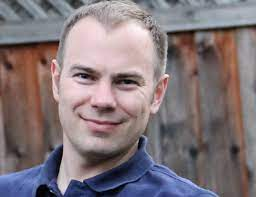
\includegraphics[width=0.4\linewidth]{chris.jpg}
\end{center}
\end{figure}
\newpage
\section*{APPLICATIONS THAT CAN BE DEVELOPED FROM SWIFT}
\paragraph{Applications that can be developed with SWIFT includes the following:
}
\begin{itemize}
	\item Facebook
	\item Uber
	\item Slack
	\item Accenture
	\item Khan Academy
	\item Lyft
	\item LinkedIn
	\item WhatsApp etc.
	
\end{itemize}
\newpage
\section*{IDE’s FOR SWIFT}
\paragraph{The Integrated Development Environments for SWIFT includes the following:}
\begin{itemize}
	\item X Code
	\item Visual Studio Code
	\item Apple
	\item C Lion
	\item App Code etc.
	
\end{itemize}
\newpage
\section*{PROGRAMMING LANGUAGES RELATED TO SWIFT}
\paragraph{These include:
}
\begin{itemize}
	\item Objective-C 
	\item Rust 
	\item Haskell
	\item Ruby
	\item Python 
	\item C sharp
	\item CLU etc.
\end{itemize}
\end{document}

